\documentclass[tikz,border=10pt]{standalone}
\usepackage{newtxtext,newtxmath}
\usetikzlibrary{positioning,arrows.meta}
\begin{document}
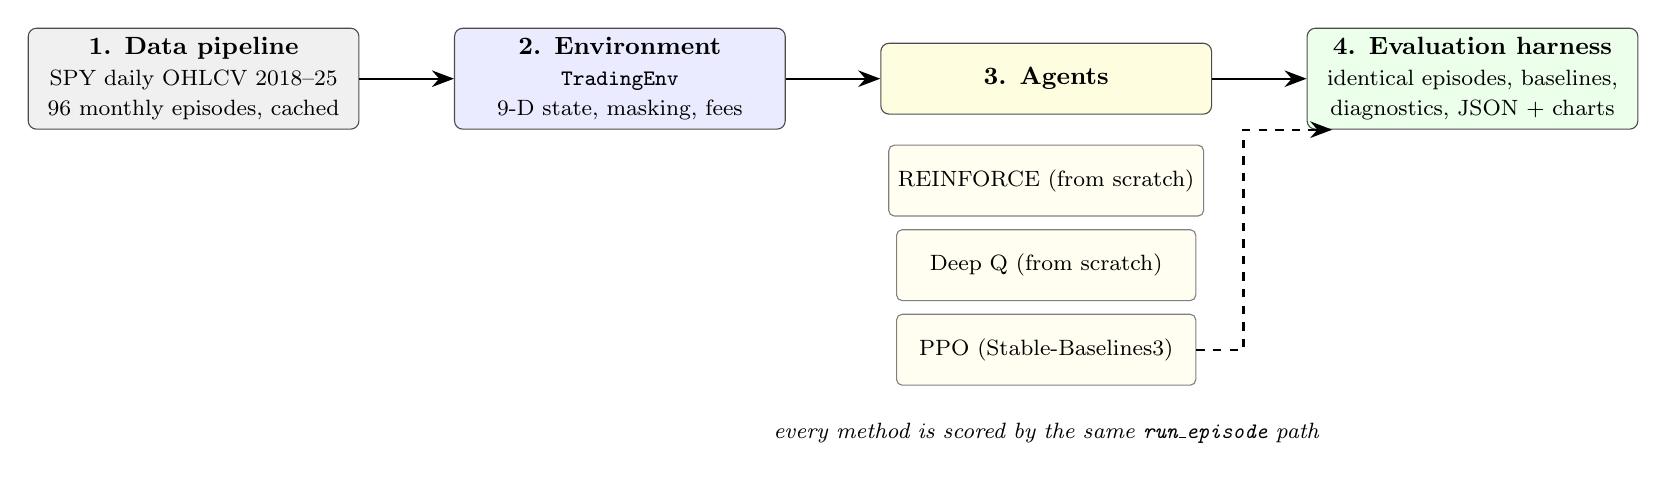
\begin{tikzpicture}[
  box/.style={rectangle, rounded corners=3pt, draw=black!70, align=center,
              minimum width=4.2cm, minimum height=1.2cm, font=\small},
  sub/.style={rectangle, rounded corners=2pt, draw=black!50, align=center,
              minimum width=3.8cm, minimum height=0.9cm, font=\footnotesize},
  arr/.style={-{Stealth[length=2.8mm]}, thick},
  note/.style={font=\footnotesize\itshape, align=center, text width=10cm}
]
\node[box, fill=black!6] (data)
  {\textbf{1. Data pipeline}\\ \footnotesize SPY daily OHLCV 2018--25\\
   \footnotesize 96 monthly episodes, cached};
\node[box, fill=blue!8, right=1.2cm of data] (env)
  {\textbf{2. Environment}\\ \footnotesize \texttt{TradingEnv}\\
   \footnotesize 9-D state, masking, fees};
\node[box, fill=yellow!12, right=1.2cm of env, minimum height=0.9cm] (agents)
  {\textbf{3. Agents}};
\node[sub, fill=yellow!6, below=0.38cm of agents] (a1)
  {REINFORCE (from scratch)};
\node[sub, fill=yellow!6, below=0.16cm of a1] (a2)
  {Deep Q (from scratch)};
\node[sub, fill=yellow!6, below=0.16cm of a2] (a3)
  {PPO (Stable-Baselines3)};
\node[box, fill=green!8, right=1.2cm of agents] (eval)
  {\textbf{4. Evaluation harness}\\ \footnotesize identical episodes, baselines,\\
   \footnotesize diagnostics, JSON + charts};

\draw[arr] (data) -- (env);
\draw[arr] (env) -- (agents);
\draw[arr] (agents) -- (eval);
\draw[arr, dashed] (a3.east) -- ++(0.6,0) |- (eval.200);
\node[note, below=0.35cm of a3]
  {every method is scored by the same \texttt{run\_episode} path};
\end{tikzpicture}
\end{document}
